Applikationen benytter tre Firebase produkter for at fungere, Authentication, Realtime Database og Storage.\\

 Firebase Auth\cite{FirebaseAuth} bruges til af håndtering brugere som login og oprettelse. Den indeholder data som Email, en hashet password og en unik identifier der bliver skabt af Firebase Authentication, når brugeren bliver skabt. Firebase tilbyder en Console , som er en web site, der giver mulighed at se og manipulere med sin data og konfigure sin Firebase.  Nedeunder kan et oversigt med informationer over brugerer ses. 
\begin{figure}[H] % (alternativt [H])
	\centering
	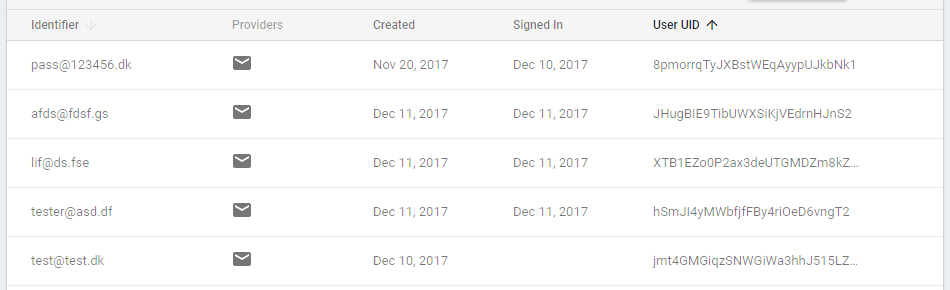
\includegraphics[height=5cm, width=15cm]{../ArkitekturDesign/Design/Firebase/FirebaseAuth.PNG}
	\caption{Oversigt over authentication data i firebase Console}
	\label{fig:FirebaseAuthPNG}
\end{figure}

Firebase Realtime Database bliver i forbindelse med applikationen vil blive brugt som en "opslagstavle", som vist nedeunder.  
 
\begin{figure}[H] % (alternativt [H])
	\centering
	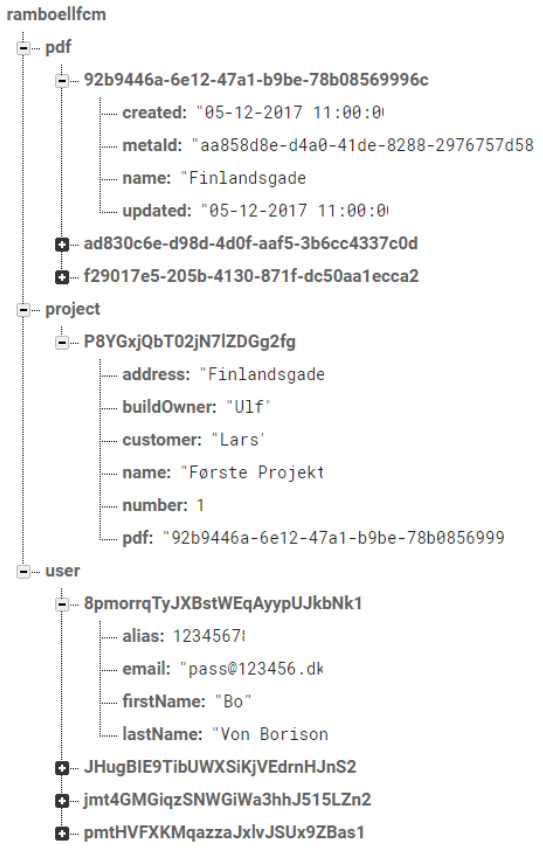
\includegraphics[height=10cm, width=10cm]{../ArkitekturDesign/Design/Firebase/FirebaseDB.PNG}
	\caption{Oversigt over database data i firebase Console}
	\label{fig:FirebaseDBPNG}
\end{figure}

På figur \ref{fig:FirebaseDBPNG} vises hvordan applikationens database er struktureret som et træ, med en root node\cite{rootNode} der hedder ramboellfcm, som derfra bliver opdelt i 3 noder:
\textbf{pdf}, \textbf{project} og \textbf{user}.\\

\textbf{Pdf} node indeholder en liste af Guid \cite{GUID}, fungerende som keys i pdf node, der bruges til at tilgå de specifikke pdf node, under hvert specifik pdf node er der 4 key-value-pair\cite{KVP}, ud over fungerer disse Guid som en referrence til Firebase Storage, når det bliver nødvendigt at hente filen ned lokalt.  Dette gør at man let kan se hvilket projekter og pdf'er der findes i databasen, og vente med at downloade PDF'en indtil når man har brug for det. På den måde kan man let få en oversigt over hvilket projekter og pdf'er der er, og kun hente de data man har rigtig behov for. 
\begin{itemize}
	\item \textbf{created}\\
	Giver en dato om hvornår denne objekt er oprettet med en nøjagtighed til sekund, der kan forhøjes hvis det føles nødvendig.\\
	\item \textbf{metaId}\\
	En referrence til json-file der er gemt i Firebase Storage\cite{FirebaseStorage}, som indeholder de objekter der skal tegnes på pdf'en. Der bliver brugt når vi skal indlæse de objekter der bliver oprettet på pdf'en.\\ 
	
	\item \textbf{name}\\
	Navnet på pdf som menneskelig læsligt tekst indtastet af brugeren, da en guid vil ikke give meget mening for brugeren.\\
	
	\item \textbf{updated}\\
	En timestamp der fortæller hvornår json-filen, som meta-filen referrer til sidst er blevet ændret. Dette bruger applikationen til at sammenligne den lokale version af json-fil med den der ligger i Storage.   
\end{itemize}

	\textbf{Project} node har den samme structur som \textbf{pdf} node af samme grund. Der er istedet for 6 key-value-pair. 
	\begin{itemize}
		\item  \textbf{address}\\
		Værdien gemt i address vil være et vej navn, der fortælller hvor projektet befinder sig.\\
		\item  \textbf{buildOwner}\\
		For diverse projekter vil der være bygge herrer, her vil der være gemt kontakt informationer til byggeherren, som navn, email og telefonnummer. \\ 
		\item  \textbf{customer}\\
		Denne key indeholder kontakt informationerne for hvem der udføres tilsynsrapport over for.\\
		\item  \textbf{name}\\
		Et menneskelig læsligt navn til projektet, for at gøre det overskulig for brugerne.\\
		\item  \textbf{number}\\
		Rambøll bruger også et projekt nummer til deres projekter, og dette sætter de selv som brugere, og derfor gemmes denne information her\\
		\item  \textbf{pdf}\\
		En Referrence til en pdf node, samt en referrence til Firebase Storage så applikationen kan  downloade PDF'en når den først har brug for det.\\
	\end{itemize}

\textbf{User} node indeholder de brugerdefineret data der tilhører brugerne af applikationen. Det id der bliver brugt som key til \textbf{user} stammer fra Firebase Authentication, og er en reference til User uid som ses på figur \ref{fig:FirebaseAuthPNG}. 
\begin{itemize}
	\item \textbf{alias} \\
	Her gemmes telefon nummeret til brugeren. \\
	\item \textbf{email} \\
	Brugerens email vil blive gemt i både Firebase- Authentication og Storage, for at gøre det let tilgænglig at tilgå det information.\\
	\item \textbf{firstName} \\
	Fornavnet på brugeren\\
	\item \textbf{firstName} \\
	Efternavnet på brugeren\\

\end{itemize}

